\subsection{Renseigner les 
profils patients}\label{diagramme-renseigner-les-profils-patients}

\begin{figure}
\centering
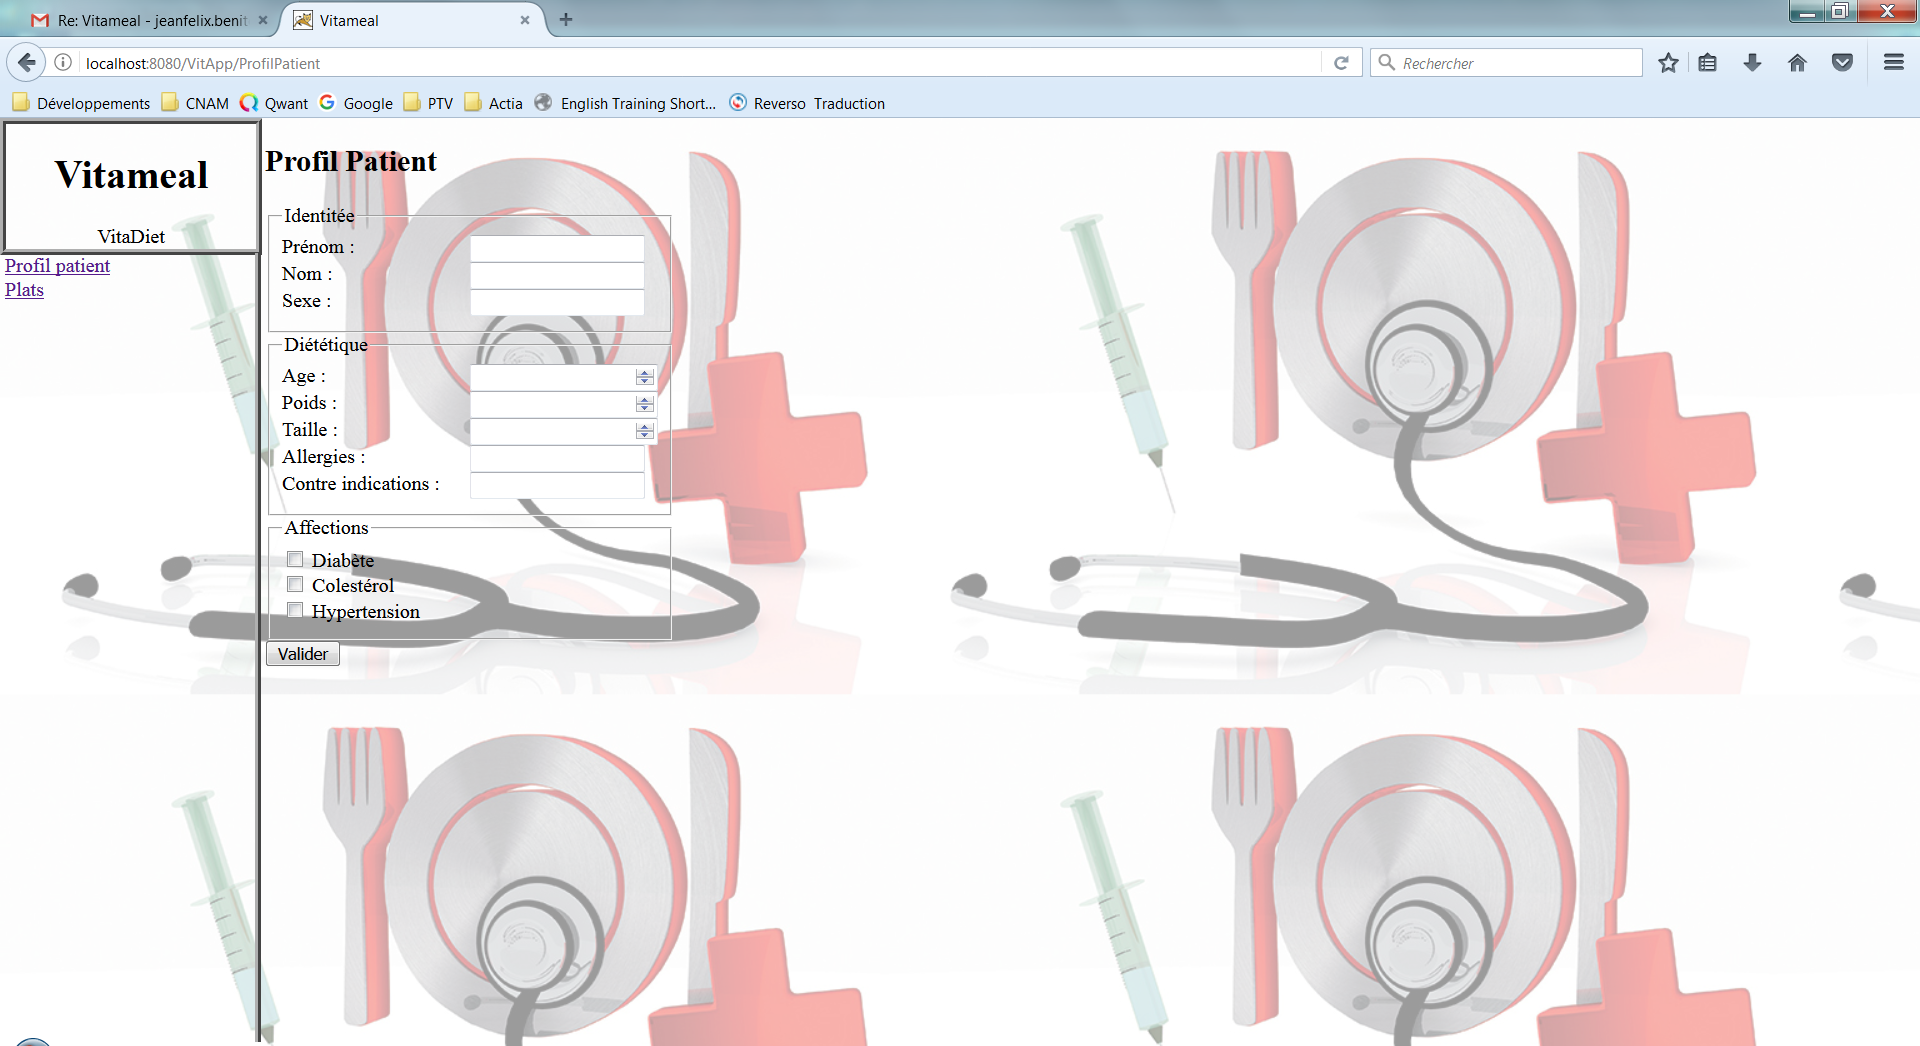
\includegraphics[width=0.9\textwidth]{../../CasDUtilisations/ProfilPatient.png}
\caption{Use case renseigner les profils patients}
\end{figure}

\subsubsection{UC300 - Renseigner les profils patients}\label{uc300---renseigner-les-profils-patients}

\noindent\textbf{Nom:} Renseigner les profils patients\\
\textbf{ID:} UC300\\
\textbf{Description :} Le diététicien souhaite pouvoir renseigner les
profils patients, en indiquant les nom, prénom, date de naissance, lieu d'hospitalisation,
régime alimentaire requis.\\
